\section{Satellite galaxies around a massive central - part 2}
The exercise is done in the script satellite2.py. The necessary explanations of the methods used are in the comments of the code. 
For question (a), we do the following: \lstinputlisting[firstline=6,lastline=138]{satellite2.py} 
The results of the maximization are in: \lstinputlisting{output_a.txt}
For question (b), we have set for all files a number of 20 radial bins. We decided not to follow any rule of thumbs, because they usually imply the sample size. 
In our case, the dataset is very large and will end up producing too many bins, which tend to give a "noisy" plot, where the pattern is difficult to be interpreted.
To guarantee readability, the bin number has been determined by visual inspection: we experimented with different bin numbers (up to 100), to end up choosing a small one
that gives a clear representation of the data, suitable for all files. We opt for a logarithmic scale, which helps visualizing a distribution which spans over some orders 
of magnitude. The range we have looking at is $[10^{-4}, 5]$, chosen after inspecting the minimum ($\sim 10^{-4}$) and maximum radii ($\sim 2.5$) values, from the observations.
The code for this part is the following: \lstinputlisting[firstline=144,lastline=508]{satellite2.py} 
We report $\langle N_\text{sat} \rangle$, the best-fit parameters $a$, $b$ and $c$ and the minimum value for $\chi^2$ found using the implemented minimization routine, which follows:
\[ \frac{\partial \chi^2}{\partial p_k} = -2 \sum_{i=0}^{N-1} \frac{y_i - y(x_i; p)}{\sigma_i^2} \frac{\partial y(x_i; p)}{\partial p_k} \]
where $y_i$ are the observations, $y(x_i; p)$ is the model depending on the parameters $p$ (in our case $a$, $b$, $c$) and $\sigma$ is the standard deviation. The sum is done 
over all the bins ($N$ is the number of data points).
The results are in:
\lstinputlisting{output_b.txt}
From these, we can see that the best-fit parameters are quite similar for all the files.
We then plot the binned observed data together with the best-fit model, for all the files (Fig.\ref{fig:fig_b}). Each file containes haloes of different masses and variable number
of satellites. In this case, we are using a Gaussian fit to data that we know follows a Poisson distribution. The Gaussian fit will introduce a bias,
by moving the mean upwards. This is because the Poisson distribution is skewed towards lower values, while the Gaussian is symmetric. Whenever the Gaussian encounters
a small value in the Poisson, it will try to compensate by increasing the mean. 

\begin{figure}[h!]
    \centering
    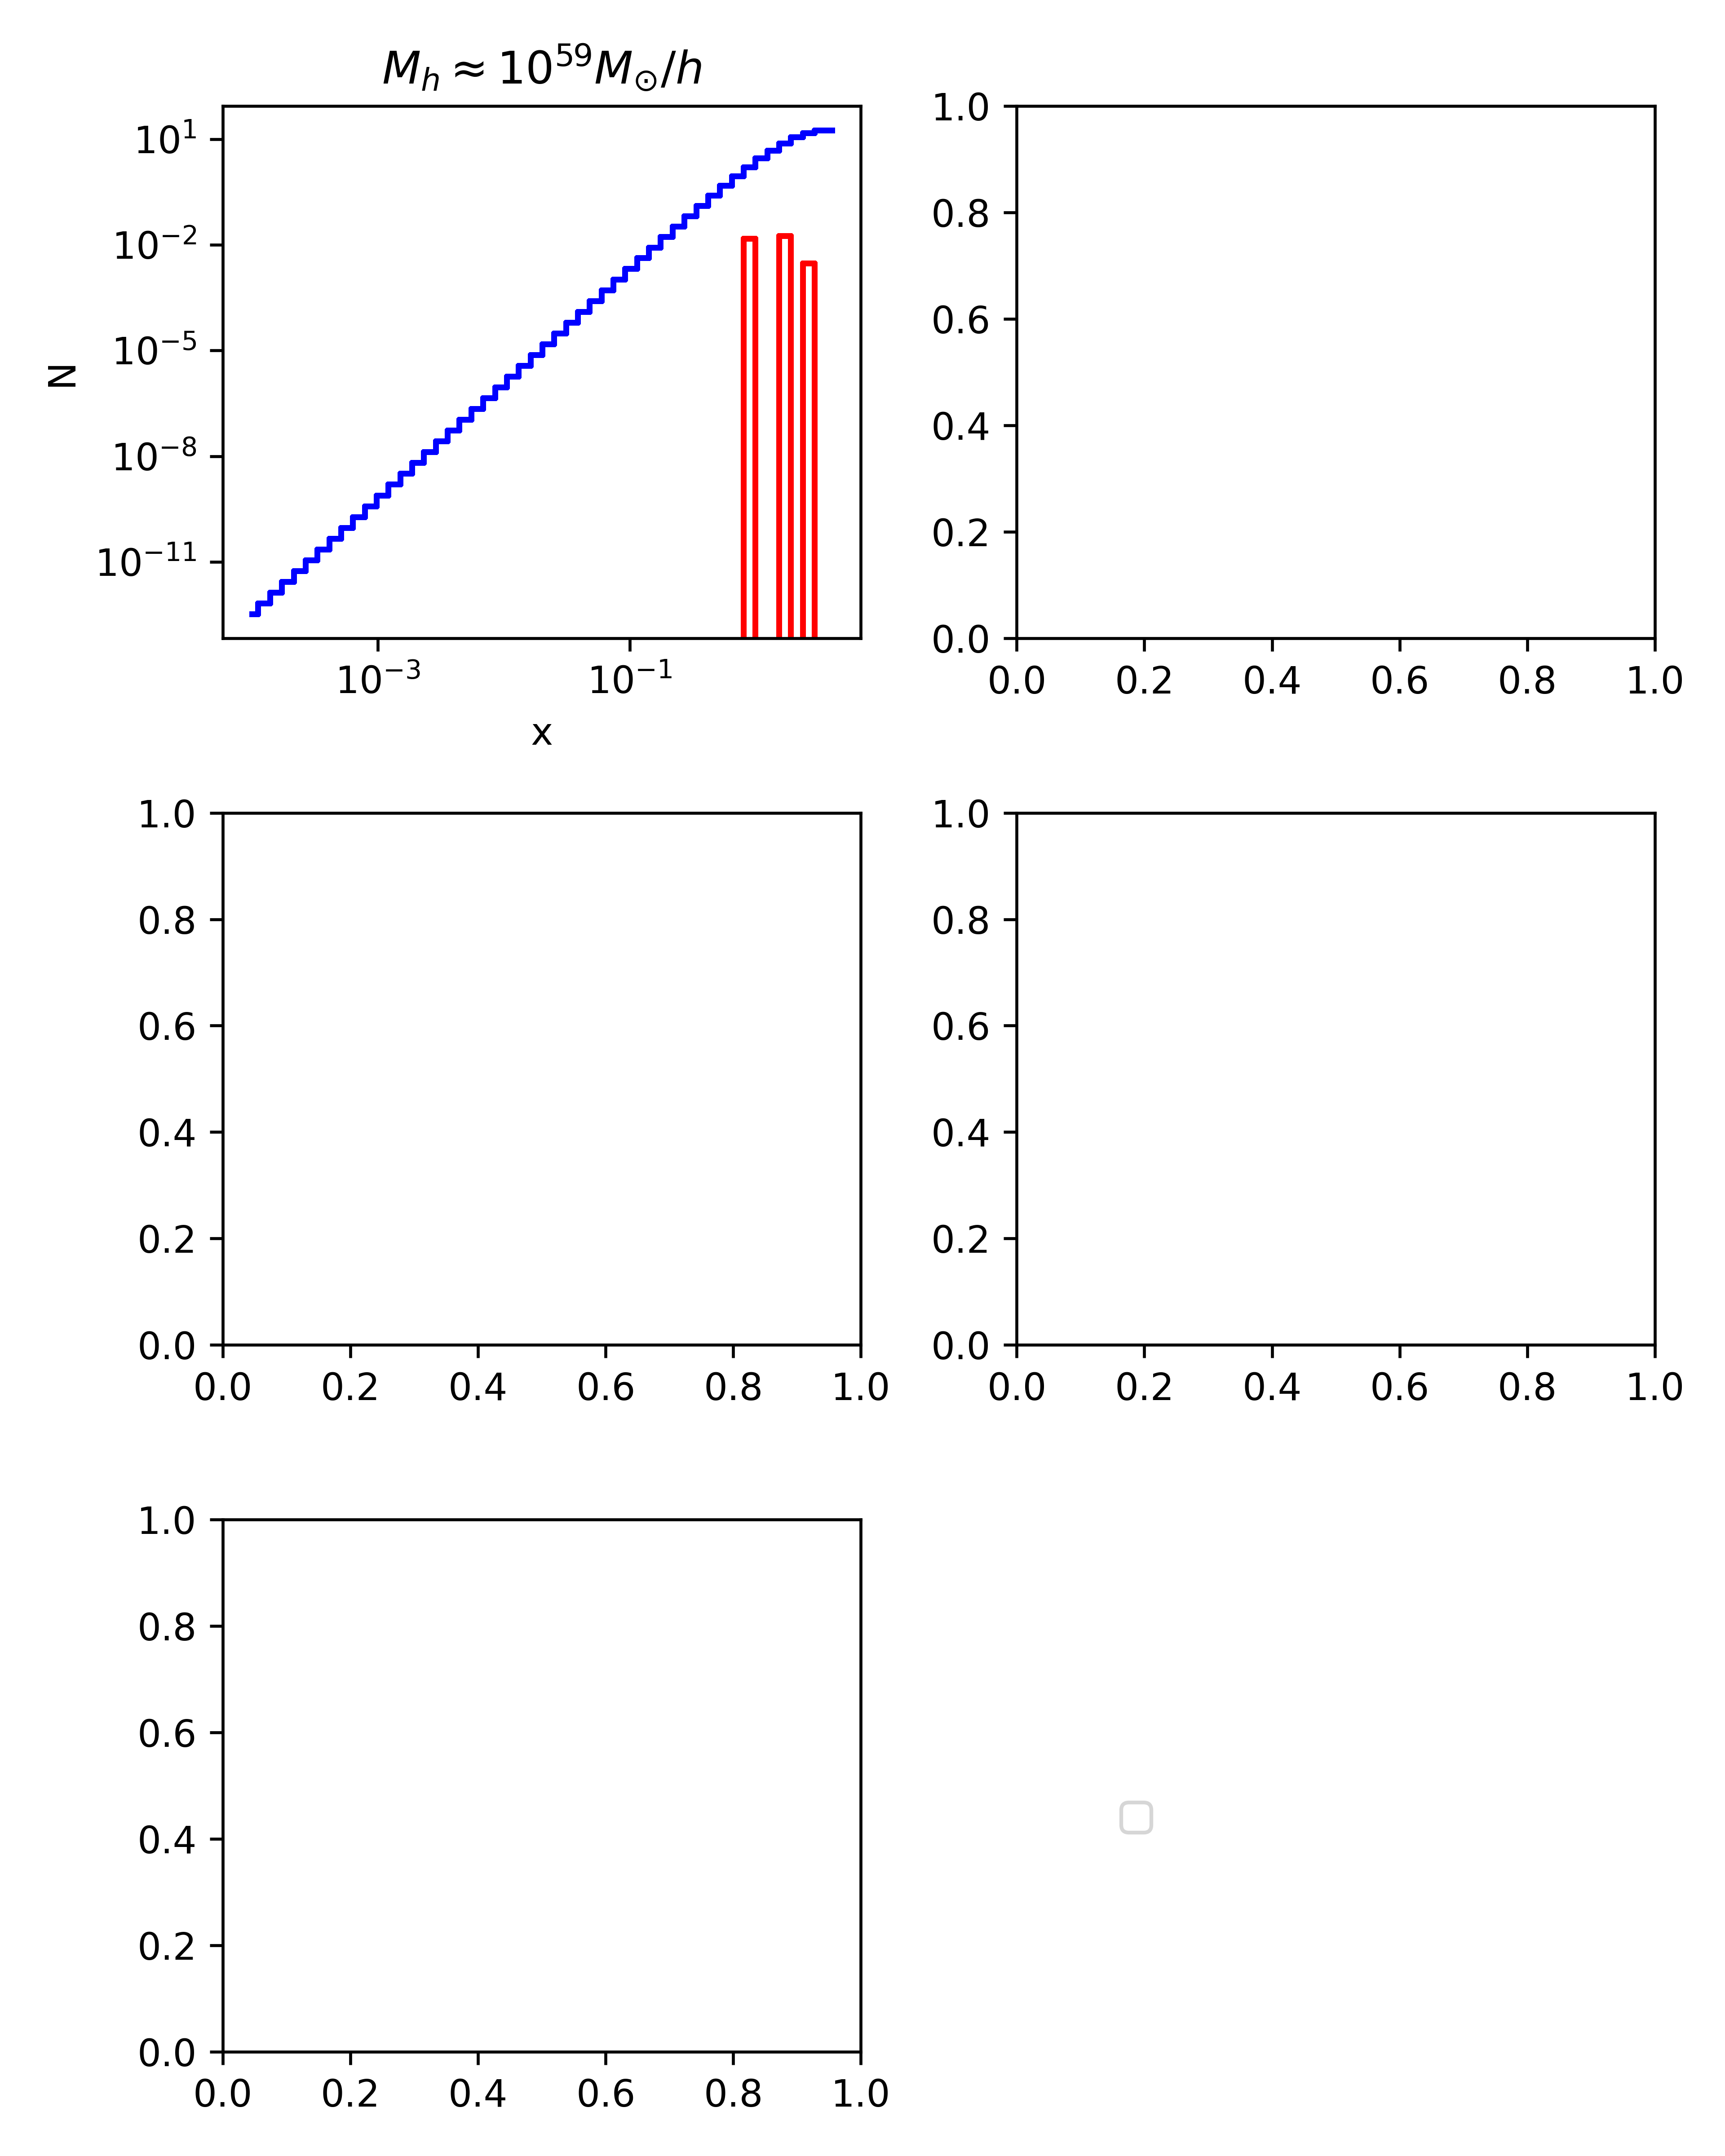
\includegraphics[width=0.9\linewidth]{./plots/my_solution_1b.png}
    \caption{Plot showing the binned observed data together with the best-fit model for all the files in logarithmic scale, in case of a $\chi^2$ approach. We have the model mean $\tilde{N_\text{i}}$ vs the radial coordinate $x$.}
    \label{fig:fig_b}
  \end{figure}

For question (c), we use the unbiased approach, with the Poisson log-likelihood:
\[ -\ln \mathcal{L}(\mathbf{p}) = -\sum_{i=0}^{N-1} \left( y_i \ln[\mu(x_i; \mathbf{p})] - \mu(x_i; \mathbf{p}) - \ln(y_i!) \right) \]
where $\mu = \tilde{N_\text{i}} =  4\pi \int_{x_i}^{x_{i+1}} \eta(x) x^2 \, dx $, i.e. the model counts and $y_i = N_i$ the mean observed counts in each bin. 
To find the minimum of the negative log-likelihood, we have followed again the conjugate gradient descent method.
We know that the derivatives of the log-likelihood are given by:
\[ \frac{\partial \chi^2}{\partial p_k} = -2 \sum_{i=0}^{N-1} \frac{y_i - y(x_i; p)}{\sigma_i^2} \frac{\partial y(x_i; p)}{\partial p_k}\]
The main difference with respect to the $\chi^2$ case is that the Poisson log-likelihood does not have the quadratic terms in the multiplying factor.
Since the derivatives of the model with respect to the parameters are the same, we adapt the computations done before by changing the factor accordingly.
The code for part (c) is the following: \lstinputlisting[firstline=512,lastline=576]{satellite2.py}
The results are in: \lstinputlisting{output_c.txt}

We then plot the binned observed data together with the best-fit model, for all the files (Fig.\ref{fig:fig_c}).  We would expect the Poisson approach to make the mean higher with respect to the $\chi^2$ fit.
Anyway, the results of part (c) are not reliable because we should have worked with discrete variables $y_i$. To do so, we thought that the data should not be divided by the number of haloes. We tried but 
the results did not seem to be correct.

\begin{figure}[h!]
    \centering
    \includegraphics[width=0.9\linewidth]{./plots/my_solution_1c.png}
    \caption{Plot showing the binned observed data together with the best-fit model for all the files in logarithmic scale, in case of a Poisson approach. We have the model mean $\tilde{N_\text{i}}$ vs the radial coordinate $x$.}
    \label{fig:fig_c}
  \end{figure}

For question (d), we have to compute the G-test statistic, to compare the goodness of fit of the two models. We have to compare the observations $O_{i}$
with the expected values $E_{i}$, which are the model counts. We want the counts observed to be integers, so we remove the division by the number of haloes.
To have a fair comparison, we have to adapt the model in a way it keeps track of how many satellites are observed, since it only gives the distribution
of the events. In this direction, the model has been scaled by a factor $ \sum_{i} O_{i} / \sum_{i} E_{i} $, which is the total number of observed satellites 
divided by the total number of expected satellites. In such way, we have that the sum of the expected values is equal to the sum of the observed values.
We chose as number of degrees of freedom $N - k$, where $N$ is the sample size (number of data points) and $k$ is the number of parameters of the model ($a$, $b$ and $c$).
A trouble we encountered is how to deal with the bins where the observed counts are zero. We tried with adding an if condition in case
the observed counts in a bin were zero, to make the G-test statistic return zero. 
The code for part (d) is the following: \lstinputlisting[firstline=585,lastline=681]{satellite2.py}
The results are in: \lstinputlisting{output_d.txt}
In case of a correct approach, these results would be helpful to understand which model is better in fitting the data. 
In our situation, the G-test statistics is probably applied on models and data which are not computed with the right logic, so the p-value is not giving any useful information.







